\newpage
\section{Additional Information}
\label{sec:04_additionalInformation}
\todo[inline]{Not sure whether I mentioned earlier: "investigate" must be uesd carefully. You can say things like: "The performance of XYZ will be investigated." (but here I would also prefer "examined"). But you certainly can not say "XYZ will be investigated" because in this context "investigate" has more of a "legal" connotation.}

On top of the direction detection by \ac{TDOA}, additional information can be
extracted from the microphone data.
This information can be used to improve the single robot result or
to feed the team filter with beta\todo{beta or better? If beta: what does it mean?} information.
As \cref{sec:03_distance} has described, the distance of the sound source
can be estimated approximately for nearby signals that are aligned with
the x-axis of the robot's head.
Another intuitive approach is the inspection of the \ac{SNR} which
is expected to be higher for closer sound sources.
In addition, the \ac{PSNR} of the \ac{GCC} as defined in \cref{sec:03_snr} is examined.

\subsection{Distance Approximation}
\label{subsec:04_distance}

\Cref{sec:03_distance} presented the necessary conditions required to estimate the
distance of the sound source on a single robot.\todo{Please check whether this
sentence still states what you wanted to say. (Are you trying to say that under
certain conditions one can estimate the distance of the sound source from
a single robot? Or are you saying that certain conditions must hold for the
single robot to compute the distance from multiple robots (e.g. single robot
has to be able to resolve ambiguity of multiple candidates.))}
To examine the validity of these assumptions, measurements from the front and
back of the robot are collected and evaluated.
\Cref{tab:04_distance} lists the true distance as well as the distance estimate
for each measurement.
For both measurements with zero distance, the orientation of the whistle differed.
180\si{\degree} indicates that the whistle was turned in the opposite direction
of the robot.
In the other case (0\si{\degree}), the whistle was aligned with the robot.
The distance is represented in robot coordinates, so that positive distance
expresses that the source was placed in front of the robot and oriented towards it
and vise versa.
\todo[inline]{Maybe it would be good to use the same convention for all
measurements here. You could either annotate all measurements with an angle and
only positive distances or have a only a sign for all measurements (omit angle
for 0 as you can simply write +0 and -0) but have an explicit sign for all
measurements ( write +0.9 instead of 0.9)}
\todo[inline]{It might be more helpful to report errors here instead of the
estimates, but it's not a big problem if you leave it like this.}
\todo[inline]{I am guessing that for measurement 1 and 2 the true distance was
6 and 9 meters rather than 0.6 and 0.9 meters? Also, is there a reason why you
have more measurements from the back than from the front?}
% -------------------------------------------------------------
\btline{ht}{1.2}
\btab{|c|c|c|c|c|c|}
\hline
Nr. & True Distance [\si{\meter}] & GCC Result [\si{\meter}] & CC Result [\si{\meter}] & Phase Result [\si{\meter}]\\
\hline
1 & 0.9 & $\infty$  & $\infty$ & $\infty$ \\
\hline
2 & 0.6 & $\infty$ & $\infty$ & $\infty$ \\
\hline
3 & 0.3 & 0.35 & 0.25 &  0.13 \\
\hline
4 & 0.0 (180\si{\degree}) & -0.13 & -0.15 & -0.23 \\
\hline
5 & -0.0 (0\si{\degree}) & 0.22 & 0.21 & 0.02 \\
\hline
6 & -0.3 & -0.15 & -0.27 & -0.45 \\
\hline
7 & -0.6 & -0.34 & -0.50 & -0.62 \\
\hline
8 & -0.9 & -0.70 & -0.91 & -0.99 \\
\hline
9 & -1.2 & -1.00 & -1.28 & -1.71 \\
\hline
10 & -1.5 & -1.39 & -1.59 & -2.98 \\
\hline
11 & -1.8 & -1.72 & -2.07 & -3.33 \\
\hline
12 & -2.1 & -2.16 & $\infty$ & -3.02\\
\hline
13 & -2.4 & -2.31 & $\infty$ & $\infty$ \\
\hline
14 & -3.75 & -3.66 & -9.51 & -4.15 \\
\hline
15 & -6.4 & -7.35 & -7.27 & $\infty$  \\
\hline
16 & -9.8 & $\infty$ & $\infty$ & $\infty$ \\
\hline
\etab
\et{Result of front and rear distance for all methods.}{04_distance}
% -------------------------------------------------------------

As the results show, that in many cases the distance can be approximated with
adequate\todo{adequate rather means something like "hinreichend/ausreichend", maybe use "adequately
small error" oder "sufficiently small error"} error. One can see that the
\ac{GCC} results are erroneous for small
distances, but gives a correct approximation steadily.\todo{What do you mean by "steadily"?}
Compared to this, the \ac{CC} method performs better for small distances,
but fails completely for some measurements.
These failures of the \ac{CC} could be mostly attributed to cases where the
lateral delays exceeded the maximum lateral samples incorrectly.\todo{What do
you mean by "exceeded incorrectly", maybe drop "incorrectly"?}
The phase method provides most incorrect results.
Especially measurement 10 stands out by being double the real value.

\todo[inline]{Maybe you can show only the error statistics here and put the
real measurements in the appendix?}

For all measurements, the resulting direction angle of the sound source were
accurate.
\todo[inline]{For all measurements and all methods? Or does this statement only
hold for GCC? It seems like CC and Phase have some wrong predictions in 12 and
13}
Furthermore, the algorithm correctly detects sources that are out of
observable range.\todo{Is this the "observable range" or should this rather be
the "relevant range" (since these bounds seem to be imposed by SPL, not in
general)}

Unfortunately, for real cases one can not rely on the height parameter of the sound
source which varies from the referee's body height.
Having this as approximation only, the distance result should be handled
with care.

\subsection{SNR}
\label{subsec:04_snr}

Estimates of the uncertainty of a measurement can be utilized to inform the
Bayesian updating algorithm.
Depending on the uncertainty, the covariance matrix of the incoming result can
be adjusted so that predictions that are assumed to have higher error have
a smaller influence to the posterior estimate.
If a relation between received signal strength and distance to the source exists,
it would be a simple way to predict the sound source position roughly.
This can help for example, when team filter intersections are clustered so that
multiple location results exist.
% Thus, one intuitive hypothesis is assuming the existence of a relation between the
% received signal strength and distance to the source.

Taking the measurements of \cref{subsec:04_labMeasurements}, this hypothesis is
investigated by looking at the relation between distance and relative \ac{SNR}.
By reason of the whistle not blown equal for all measurements,
the \ac{SNR} is scaled by the overall mean of all robots' \acp{SNR} for one
measurement.
% $\text{Relative SNR} = \frac{SNR_{robot}}{Mean(SNR_{measurement})}$.
In \cref{fig:04_snrDistance} no straightforward
link between both values can be found unexpectedly.\todo{I would not write
"unexpectedly" here.}
\todo[inline]{Maybe report the correlation of these measurements. You can then
say, that SNR and Distance are only weakly correlated (small rho) which is
a bit more precise that using the "optisch gefuehlte Korrelation".}
% -------------------------------------------------------------
\begin{figure}[ht]
	\centering
	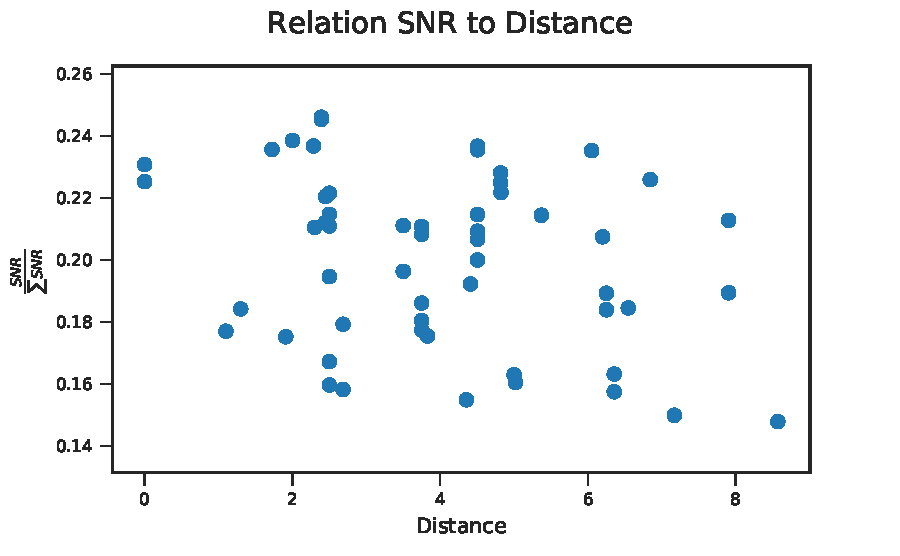
\includegraphics[]{figures/evaluation/snr_scatter}
	\caption{Visualization of relation between SNR and distance.}
	\label{fig:04_snrDistance}
\end{figure}
% -------------------------------------------------------------

Due to the result, further analysis on the \ac{SNR} values
on individual robots is done for evaluation of the microphones' validity.
\todo{How does this relate to your last sentence above? (I thought that the
conclusion was that things don't correlate?)}
For this purpose, a signal is played back digitally from fixed distance
and constant volume with different angles.
The main purpose of this measurement is to ensure that the individual channels
are not biased.\todo{Biased towards what?}
14 measurements of a 3\si{\kilo\hertz} sine signal
with are distance of 0.73\si{m} are done but no tendency is detectable.
Further evaluation is done by determining the channel with the maximum
\ac{SNR} of one measurement.
It is expected that the nearest channel to the sound source has maximum \ac{SNR}.
At 85.71\si{\percent} of the measurements this assertion could be
evidenced.\todo{How many measurements did you take?}
From this, it can be said that the general recordings of the microphones
are neither biased nor falsified.\todo{What do you men by falsified here?}
\todo[inline]{From the number of comments I put to this section I would
conclude that you could add a little bit more details on what the purpose of
this measurement was.}
\todo[inline]{IMHO a good practice is to report the number of experiments
and/or have the data in the appendix (if you still have the data). But having
it in the appendix is not super relevant. Don't waste time on it.}.

The same procedure is done with the real whistle recordings of the
measurement in \cref{subsec:04_labMeasurements}.
Using these measurements, only 54.55\si{\percent} of the maximum \acp{SNR}
match with the expected channels.
Consequentially, one must assume that the environmental circumstances
like multi-path propagation and reflection have large influence
on the signal data.
Thus, neither for a single robot direction result nor for the team filter
the \ac{SNR} can be utilized.

\subsection{PSNR}
\label{subsec:04_psnr}

As referred in \cref{sec:02_gcc}, the main characteristic of the \ac{GCC-PHAT}
algorithm is the emerging sharp peak.
In conclusion, one can assume that the lack of a sharp peak indicates
a less valid delay result of the \ac{GCC}.\todo{What is the reasoning behind
this conclusion? Maybe it is obvious to GCC familiar people but I fail to see
the causality.}
\todo[inline]{From this section introduction it is not clear what is happening in
this section. Maybe add a sentence on what is going to happen in 4.2.3 PSNR}

\subsubsection*{Informative Value}

This statement is examined by comparing the \ac{PSNR} value
to the error of the direction angle resulting from the \ac{GCC-PHAT} delay.
% Two cases of errors are taken into consideration.
In the following, the \ac{PSNR} is referred to as high if it exceeds 17.5
whereat the \ac{PSNR} value ranges from 10.1 to 28.8 for measurements in
\cref{subsec:04_labMeasurements}.

\todo[inline]{"Firstly" can not be used like this (it means "erstens" not
"zunaechst/zuerst"). Maybe grep through the document to make sure you don't use
it.}
First, for each channel pair the error between true direction and the most
suited direction candidate\todo{most suited according to which metric? The one
that is closest to the true direction or the one that has the "sharpest peak"?}
emerging from the \ac{GCC} delay.
The results are grouped into two classes based on the associated \ac{PSNR} value.
If the \ac{PSNR} of the \ac{GCC} is greater than the threshold of 17.5,
the \ac{RMSE} of its result is grouped to the errors with high \ac{PSNR}.
Elsewise, it pertains to the errors with low \ac{PSNR}.
This valuation is done with the measurements of \cref{subsec:04_labMeasurements}
and manually set start indices.
\todo[inline]{Maybe rather:"Out of a total number of X measurements,
Y correlations reported a PSNR below the threshold. The RMSE within this group
was 35.77\si{degree}".}
Having 76 correlations assessed with low \ac{PSNR}, the \ac{RMSE} of this group
is 35,77\si{\degree}.
Compared to this, the \ac{RMSE} of the remaining 144 measurements
is 15.86\si{\degree} only.
\todo[inline]{Always report what the RMSE belong to. E.g. here I can only
conclude from the unit that these are errors on the phase. But the context
sounds like they are errors on the PSNR.}

To see the impact on a complete robot result, the same is done
with the final angular errors of single robots results.
Here, the \ac{RMSE} of the lower \ac{PSNR} case results in 25.36\si{\degree}
whereat the error of the other case is 14.41\si{\degree}.
From this correlation between PSNR value and prediction accuracy one can
conclude that the PSNR is a useful indicator to inform about the validity of
direction estimates.\todo{Make sure that this sentence still says what you want it
to say.}

\subsubsection*{Frame Selection}

Another perspective is to include the PSNR information into the single
robot whistle direction estimation.
In \cref{fig:04_psnr2FrameShift}, the frame to investigate is
shifted before and after the signal start index.\todo{Signal start marked manually?}
Here, the same measurement as in \cref{sec:04_tdoaSingle} is used where
the robot was positioned at the center point
while the whistle is blown at -33.7\si{\degree} with 4.5\si{\meter}
distance.\todo{I would not cross-reference to another section here. Just
explain the experiment setup again as if it was a stand-alone experiment.
Jumping to other sections is annoying for the reader and it is not relevant to
know that you used the exact same data.}
The frame size of the \ac{GCC} is set to 256 samples and the shift
was set to a quarter of the frame size.
Samples of the rear left channel are plotted for better understanding
in the upper graph of \cref{fig:04_psnr2FrameShift}.\todo{Why "rear left" if
the signal comes from front right?}
The second graph shows the \ac{RMSE} of the robot direction result
over the frame shifts.
For the lower graph, the mean over the \acp{PSNR} of all channels
is presented.
As a general trend, it can be observed that the error of the predicted
direction is low for frame shifts with a high \ac{PSNR}. This again confirm the
hypothesis stated early in this section.
For shifts smaller than -2, the whistle signal does not intersect with the
evaluated frames. Therefore, the prediction error in this regime is high.
An important notice is that the \ac{PSNR} decays as the frame is shifted towards
later samples on the whistle signal. This indicates that the implemented
\ac{GCC-PHAT} method is not suitable for arbitrary subsamples of the signal.
% Without additional information about the rough direction,
% ambiguity exists due to periodicity of the signal.
% Due to the inconclusive result of the \ac{SNR} in \cref{subsec:04_snr}
% one decides not to take the signal magnitude as such information
% into account.
% Thus, the decisive role of the start of the signal is underlined again.
% -------------------------------------------------------------
\begin{figure}[ht]
	\centering
	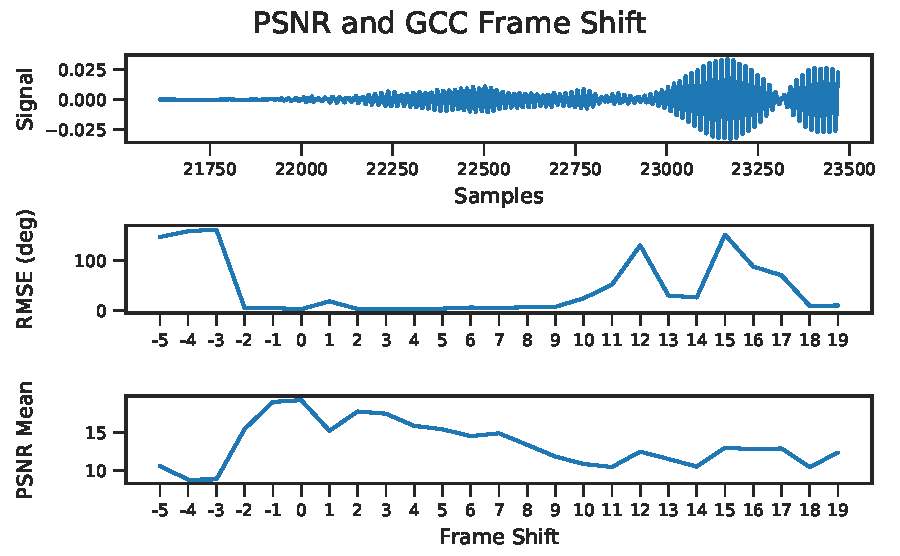
\includegraphics[]{figures/evaluation/gcc_frame_shift}
	\caption{
		Relation between \ac{PSNR}
		and selection of the frame in time. Signal data
		of the rear left channel is plotted in the upper window.
		In this measurement, the whistle is positioned at right front
		of the robot.
	}
	\label{fig:04_psnr2FrameShift}
\end{figure}
% -------------------------------------------------------------

\todo[inline]{Do you ever explicitly say how you end up using this information
in the team filter?}
